\subsection*{Database}
Systemet skal som nævnt i kravsspecifikationer have forbindelse til en database. Denne kan tilgås fra den tilhørende controller. Klasserne for databasen og controlleren fremgår af \autoref{fig:MVCDatabase}. 

\begin{figure} [H]
\centering
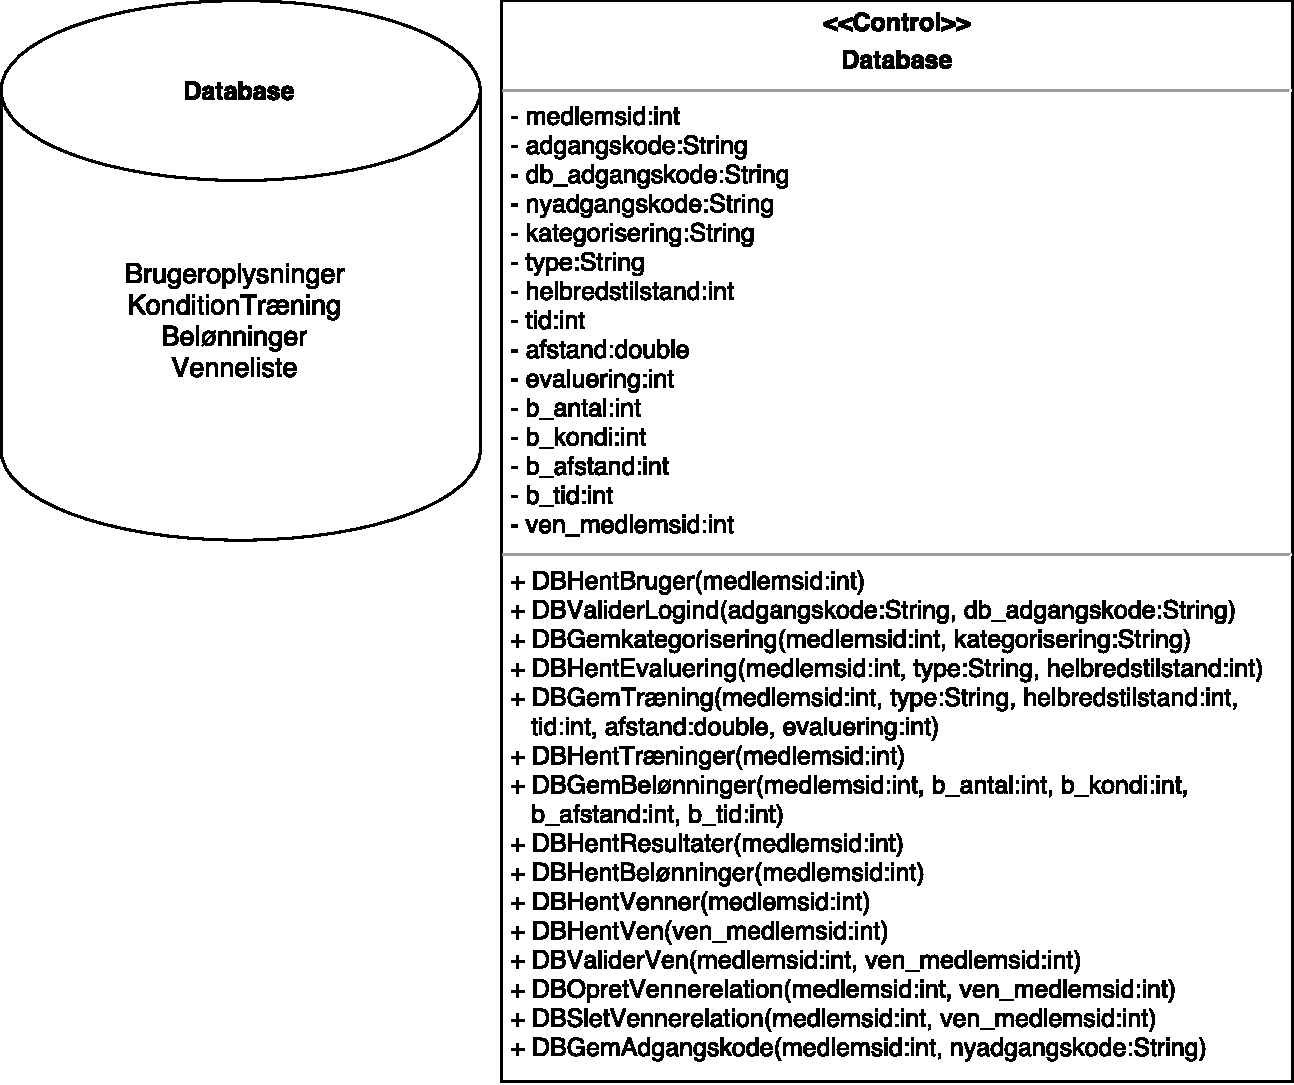
\includegraphics[width=0.5\textwidth]{figures/MVC/MVCDatabase}
\caption{Designklasse for Database. Til venstre ses databasen og til højre ses den tilhørende controller.}
\label{fig:MVCDatabase}
\end{figure}

\noindent
Databasen indeholder Brugeroplysninger, Venneliste,KonditionResultater og Belønninger. Brugeroplysninger indeholder alle brugerens oplysninger. Disse registreres i forbindelse med rehabiliteringsforløbet af sundhedspersonalet, som senere kan tilgå disse og redigere i brugeroplysningerne. Vennelisten indeholder andre bruger som brugeren følger, derudover har brugeren mulighed for at tilføje flere brugere til sin venneliste. KonditionResultater indeholder brugerens resultater for konditionstræning. Sundhedspersonalet og har mulighed for at tilgå alle resultater. Belønninger indeholder de belønninger som brugeren har opnået i forbindelse med træning. Brugeren og de brugere der følger denne har adgang til disse.  

Designet af databasen er yderligere beskrevet i et ER-diagram, der vil fremgå af \autoref{sec:ER}. \textit{Database} controlleren indeholder metoderne Hent, Valider, Gem, Opret og Slet. Disse har til formål at kommunikere mellem databasen og de forskellige controllere. Der oprettes forbindelse til databasen ved log ind, træning, resultater, venneliste samt redigering. 

\subsection*{Lagring af data}  \label{sec:entity}
Når der oprettes forbindelse til databasen i forbindelse med, at brugeren logger ind eller tilgår resultater på app'en, sendes og gemmes data i forskellige entitys, som fremgår af \autoref{fig:MVCEntity}. Der er valgt at udarbejde entitys for ikke at skulle tilgå databasen hver gang data skal hentes. Dertil er det også muligt at opdele data, som har med en specifik controller at gøre, så irrelevant data undgås. 

\begin{figure} [H]
\centering
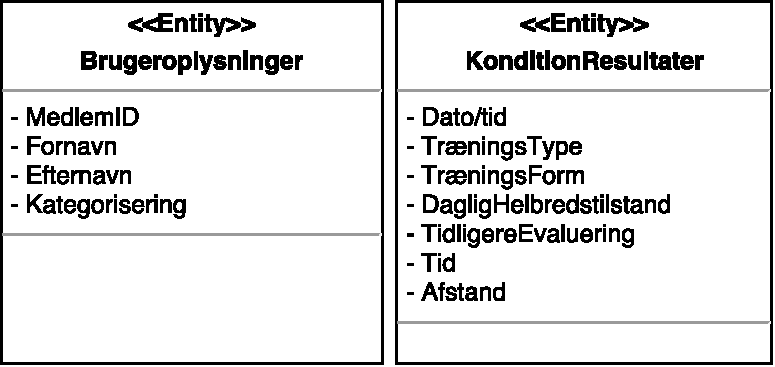
\includegraphics[width=0.5\textwidth]{figures/MVC/Entity}
\caption{Designklasser for Entitys, herunder Brugeroplysninger og Resultater. Attributterne er markeret med \#, hvilket indikerer, at disse er beskyttede.}
\label{fig:MVCEntity}
\end{figure}

\noindent
På \autoref{fig:MVCEntity} fremgår det, at de forskellige attributter er beskyttede. Dette er gjort, da det ønskes at attributterne kun kan tilgås indenfor det samme projekt. 
\textit{Brugeroplysninger} indeholder informationer om brugeren, herunder MedlemsID, Adgangskode, Fornavn, Efternavn og Kategorisering. 
\textit{Resultater} indeholder brugerens resultater, som er defineret ud fra DatoTid, TræningsType, TræningsForm, DagligHelbredstilstand, TidligereEvaluering, Tid, Afstand og Belønninger. 
